% --------------------------------------------
%		CAPITOLO 3 
%---------------------------------------------
\chapter{VTX detector}


This chapter focuses on one of the four proposals for the vertex detector upgrade of Belle II, that is VTX. After a brief reference to the reasons behind the vertex detector upgrade, we will go trough VTX concept and layout, designed with a new geometry with respect VXD and also with a different mechanical structure and new pixel sensors (OBELIX), needed to fullfil the new requirements dictated by new environment conditions. Moreover all ongoing studies are supported by continual tests and simulations that we will also take a look at.


%---------------------------------------------
%			3.1
%---------------------------------------------
\section{VTX Layout and mechanical structure}

In~\autoref{sec:nano_beam} we have introduced in a few words the concept of the \textit{nano-beam} scheme, which could allow to achieve the new fixed target of istantaneous luminosity. This new strategy required a strong focusing of the beams in particular at the IP, resulting in a large amounts of beam induced background and as consequence in a higher dose of radiation in the innermost detector layers. Therefore they have to be robust enough to keep good performance against these new hard conditions.
Furthermore to be able to increase the luminosity, SuperKEKB might have to consider an improvement of the final focusing magnets and so a potentially re-design of the interaction region, including the detector but independently of its hit rates and radiation hardness issues.\\

\begin{figure}[h!]
\centering
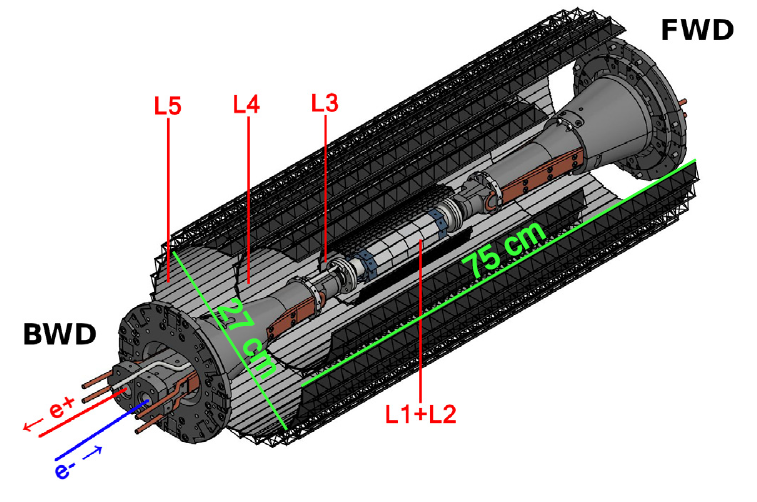
\includegraphics[scale=.6]{VTX_layers}
\caption{Concept of VTX layout with 5 barrel layers, filling the current VXD volume.}
\label{fig:VTX_layers}
\end{figure}


VTX project aims to replace the all VXD with a fully pixelated detector based on Depleted Monolithic Active Pixel Sensors (DMPAS) arranged on five layers at different distance from the beam pipe. Actually the radii and the number of the layers are currently subject to several  studies and simulations, in order to achieve an optimized arrangement (\autoref{fig:VTX_layers}). 
For now two layers are planned in the innermost part (\textit{i}VTX) and three in the outermost (\textit{o}VTX). The active lenght of the ladders is expected to vary from 12 to 70 cm to cover the required acceptance of $17^{\circ} < \theta < 150^{\circ}$.\\
As already discussed for other upgrade proposals, it is important to try to reduce the material budget, in order to minimize the multiple Coulomb scattering which particularly affects the very soft particles produced in Belle II collisions. By using a single sensor type, it is expected a reduction of the overall material budget up to 2\% of radiation lenght, against the present 3\% of VXD, which uses two different sensors such as pixels and strips.


\subsection{iVTX}

The \textbf{\textit{internal}VTX} consists of the first two detector layers devised togheter with a self-supported air-cooled all-silicon ladder concept, where four contiguous sensors are diced out of a wafer, thinned and interconnected with post-processed redistribution layers. They are designed to be at 1.4 and 2.2 cm respectively from the beam pipe, and target an individual material budget of about 0.1\% radiation lenght. 
This is actually achivable because the overall surface of these layers is moderate, below 400 $cm^{2}$, as well as low sensor power dissipation is expected to be low and the connections needed for the operation to be a few. Precisely for these reasons, air cooling could be a workable system to avoid overheating.


\begin{figure}[h!]
\centering
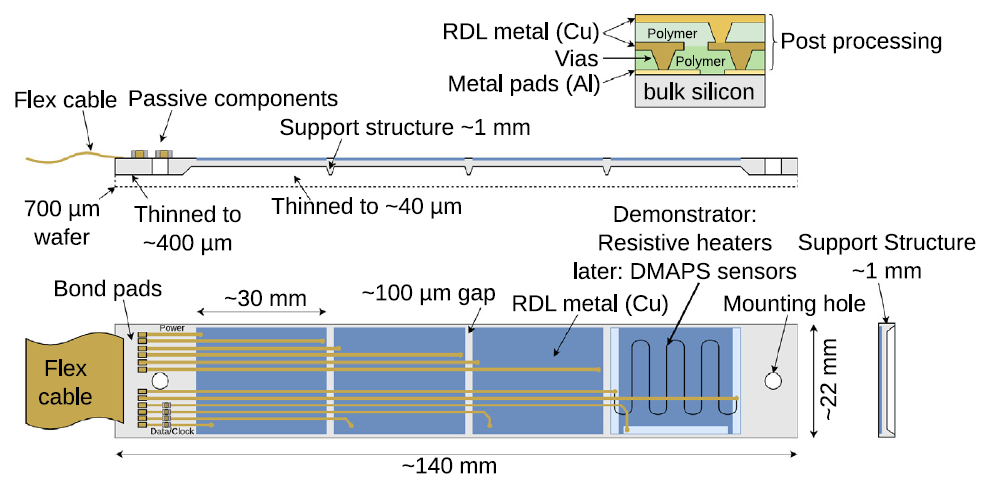
\includegraphics[scale=.65]{iVTX}
\caption{Sketch of the all-silicon ladder concept of the iVTX. Four dummy sensors are shown in blue on the silicon support in grey. The yellowish lines instead, indicate power and data transmission lines. Power is delivered to the ladder by a flex cable, which also transmits data to and from the chips in the final one.}
\label{fig:iVTX}
\end{figure}

The ladder has to be equipped with four of the aforementioned OBELIX chips and thinned to 50 $\mu$m except in some border regions, where a few hundreds of $\mu$m are necessary to ensure mechanical stability. 
In order to interconnect the sensors along the ladder and provide a unique connector at the backward end, during the post-processing metal strips are etched on the redistribution layer (RDL). The latter has the main purpose to route power and data via impedence-controlled transmission lines to a flex cable, added at the end of the ladder.
After the RDL processing, the backside of the ladder has to be thinned in accordance with what was previously mentioned. Mounting holes will be added via laser-cutting.


In~\autoref{fig:iVTX} is showing a sketch of the iVTX demonstrator ladder (currently under production), 140 mm long and 22 mm wide (grey). Instead of the actual sensors, it is equipped with four dummies chips with a lenght of about 30 mm (blue), which are used as resistor to mimic the estimated heat load in order to test the air cooling system and more generally to characterized the electrical, mechanical and thermal performance of the ladder.
A redistribution layers for power and data is also added to the demonstrator, in order to connect the chips with a flex cable at the end of the ladder (yellowish lines). In addition the wafer is thinned to 400 $\mu$m and the sensitive areas down to 40 $\mu$m with the purpose to test the mechanical integrity of the whole structure.

\begin{description}
\item \textbf{R\&D}
\end{description}

The R\&D is ongoing and the full-silicon ladder concept is currently being assessed with industrial partners. First thinned ladders have been produced and characterised with different thickness and geometry.%, revealing a homogeneous thickness over an area of 10 $cm^{2}$. 

In addition several tests are focused on evaluating power delivery efficiency, the quality of the signal which travel through the ladder and also the process used to fully assembly it. 
In~\autoref{fig:iVTX_eye} are shown eye diagrams from simulation with a transfer rate of 640 Mbps, which may imply that 320 Mbps of data rate will be possible.

\begin{figure}[h!]
\centering
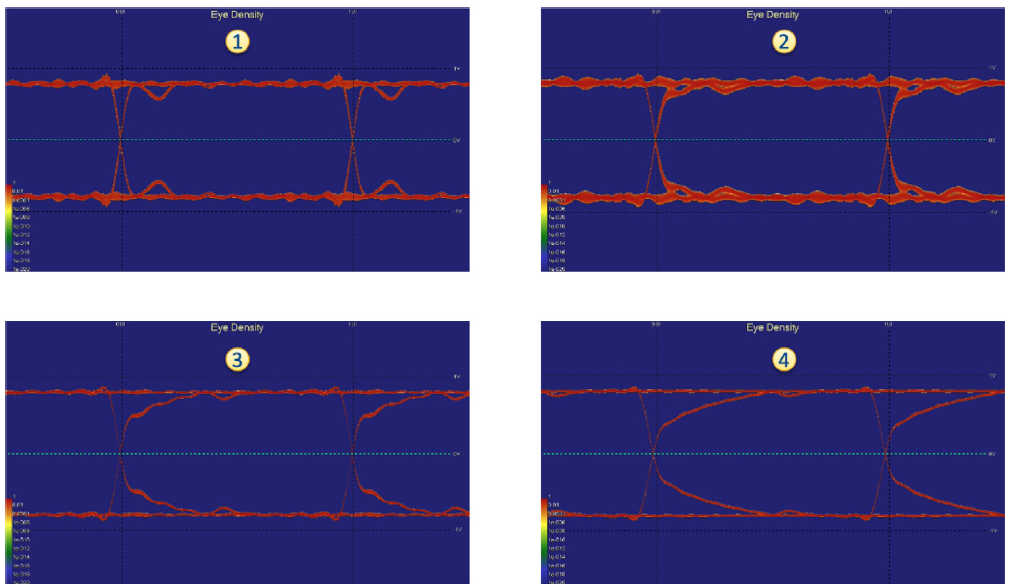
\includegraphics[scale=.7]{iVTX_eye}
\caption{Eye diagrams of the iVTX data transmission lines at four different locations on the ladder.}
\label{fig:iVTX_eye}
\end{figure}

Moreover it has been demonstrated that air at the temperature of $15^{\circ}$ and flowing with a speed of 10 m/s succeeds to cool a single inner module, assuming power is uniformly dissipated on the sensor surface. The maximum temperature reached is $20^{\circ}$C. 

Through very first estimates it is expected that an equivalent section of 6 tubes with 10 mm of diameter is necessary to expel the heat from the inner layers, roughly equal to 65 W. So it is necessary to design a mechanical structure which forseens the space needed to the tubes in order to bring the air at the IP and also compatible with the new interaction region.


\subsection{oVTX} \label{sec:oVTX}

The \textbf{\textit{outer}VTX} consists of three layers respectively at radii of 39 or 69, 89 and 140 mm from the beam pipe and because of the larger distance required to cover the acceptance, they are not self-support. They follow a more traditional approach, strongly inspired by the designed developed for the ALICE ITS2. Each ladder is water cooled and made of a light carbon fiber support structure, called \textit{truss}, which provide the mechanical integrity. Its structural design is showed in~\autoref{fig:oVTX}: 70 cm long and 5.8 g of weight, it is able to support more than 40 sensors in two rows next to each other with a small overlap, earning a material budget of 0.3\% $X_{0}$ for the first two layer and 0.8\%$X_{0}$  for the outermost one.

\begin{figure}[h!]
\centering
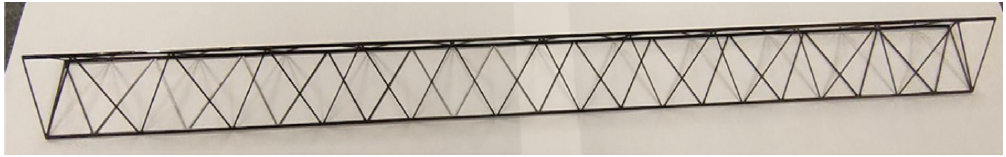
\includegraphics[scale=.7]{oVTX}
\caption{Prototype of the layer 5 \textit{truss}, which is the longest, made from thin carbon fibre structures.}
\label{fig:oVTX}
\end{figure}


For the cooling of the ladder a cold-plate concept is under development (\autoref{fig:oVTX_coldplate}), on which the sensors are glued and that in turn is installed on the truss. For each row there is a polymide cooling tube that runs over all the sensors and turns back at the other end, so that the heated coolant leaves on the same side. Then two flex print cables connect the two halves of the ladder to the connector.


\begin{figure}[h!]
\centering
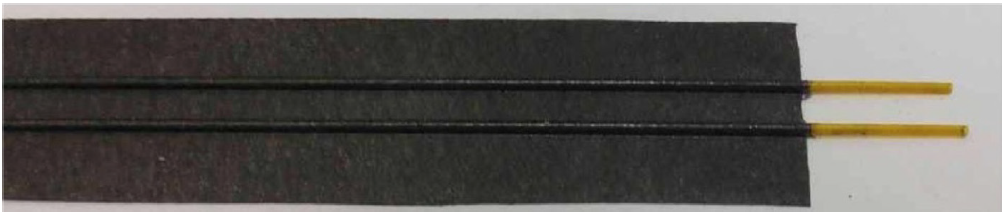
\includegraphics[scale=.7]{coldplate}
\caption{A prototype of the cold-plate for colling. One coolant tube(golden) is connected to the cold plate(black) and turns 180° on the other end (not shown) so that the coolant flows in both directions and thus leaves on the same side it starts.}
\label{fig:oVTX_coldplate}
\end{figure}

For layer 3 instead, only one flex print cable in the backward side is considered in order to leave more space in the forward for other possible services and accelerator components. In addition for the third layer two different solutions are under study: at radius of 39 mm e 69 mm respectively. 
In~\autoref{fig:ladders} are displayed schematic examples of some hypotheses. 

\begin{figure}[h!]
\centering
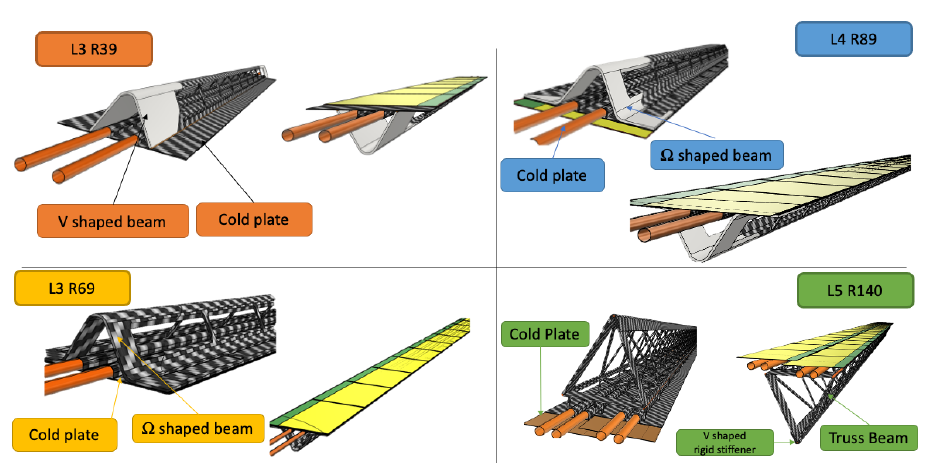
\includegraphics[scale=.7]{ladders}
\caption{Schematic view of possibile solutions for the three outermost layers.}
\label{fig:ladders}
\end{figure}


In~\autoref{fig:oVTX_5} are shown the several substructures described before, that shape a ladder of the outermost layer 5. From bottom to top come in succession the carbon fibre structure, two cold-plates for the two neighbouring sensor rows (Chips, in grey) and the flex cables for power and data transmission (green). 


\begin{figure}[h!]
\centering
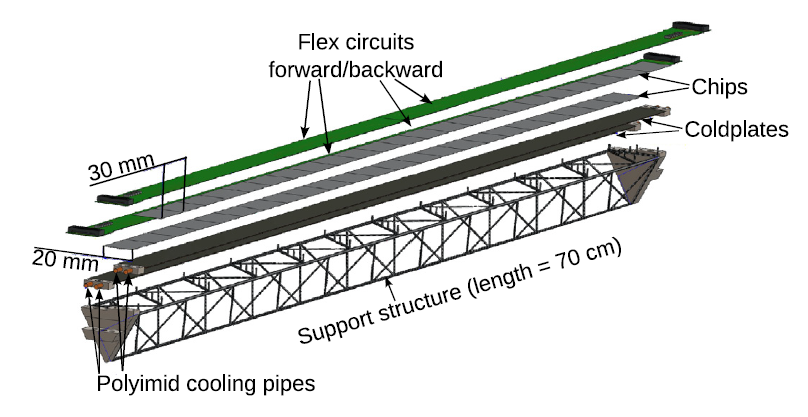
\includegraphics[scale=.7]{oVTX_5}
\caption{An exploding drawing of a fully assembled layer 5 ladder.}
\label{fig:oVTX_5}
\end{figure}

\begin{description}
\item \textbf{R\&D}
\end{description}

The carbon fiber support structure and flex cable have been designed and fabricated for the last ladder, which is also the longest. Also services for the last two ladders, like electrical connections and cooling, can be provided both on forward and backward sides.
A Multiline Power Bus has been realized in order to power each OBELIX chip along the ladder by a dedicated VDD and GND pair. \\

After the assembly described in the previous, first thermo-mechanical tests were performed and they show that the first resonance frequency is at 200 Hz, which is safely far from the one of the typical earthquakes in Japan and also that the thermal properties are good.\\

Trying to reduce as much as possible the material budget, the transmission lines and the flex cables has to be as thin as possible, but also need to ensure safe data transmission. Trace widths are trimmed to fulfill the same maximum voltage drop requirement (200 mV) for all the chips.

For this reason, the outermost ladders long 70 cm are equipped with two flex cables, one from each side of the \textit{truss}. In~\autoref{fig:oVTX_eye} the resulting eye diagram from testing the signal integrity of one of the 35 cm long transmission lines for data transmission rate of 500 Mbps. This result demonstrates that the bandwidth is large enough to allow more then needed 160 Mbps for data transmission.


\begin{figure}[h!]
\centering
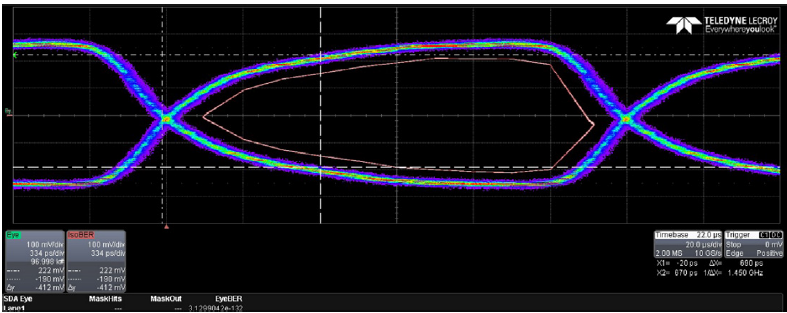
\includegraphics[scale=.8]{oVTX_eye}
\caption{Eye diagram for the oVTX transmission line signal integrity of the layer 5 flex cable.}
\label{fig:oVTX_eye}
\end{figure}


In addition, thermal tests have been performed for the last layer prototypes using kapton heaters to emulate the power dissipation of the chips. The coolant (demineralized water) has been set to a temperature of $10^{\circ}$ at the beginning, the environment at $20^{\circ}$ with a negative pressure 0f 0.2 bar. Results have been demonstrated that for three different configurations of the flow (such as monodirectional, bi-directional and with an U-turn at one end) the average temperature stands at $24^{\circ}$ with a maximum gradient of $\Delta T \approx 4^{\circ}$ along the full lenght of the ladder. 

All these test validate the design of the longest ladder, which is indeed the most challenging, and therefore the possibility to operate the chips safely.


\subsection{Thermomechanics and data transmission}

The proposed VTX detector intends to employ the same sensor type for all the layers in order to use a unique control and power supply system. It is expected to operate at room temperature and for what we have seen in the previous, the smaller cross section of data cables, the usage of optical fibers and the less complex cooling system might allow a considerable reduction of services with respect to the current VXD. This allows more room for maneuver in the design of the new IR, needed for ramping up the istantaneous luminosity in the future.

As consequence also the design of the mechanical support system, data cables and acquisition system required could be more simple and in particular, the standard PCIe40 acquisition boards used in Belle II match well the data throughput requirement.

%---------------------------------------------
%			3.2
%---------------------------------------------
\section{Performance simulation}
%richiesta sensitivity di 150 um ? VTX article, betagamma

%Accennare a problemi CDC?
%\ref{} to chapter 2

As we have seen in chapter 2, the experiment aims to reach a new peak of luminosity in further future, but it has to face also the consequences, like the higher level of machine related background and so larger doses of radiation, expecially in the inner layers of the whole detector. 
For this reason a lot of simulations and studies are focusing on ensuring that the main physics goals of the experiment will be achieved despite the more severe conditions to which it wuold be subjected. 

The VTX upgrade program wich foresees for a new silicon vertex detector with high granularity in both space and time, could bring significant improvements in tracking efficiency expecially at low momentum, in the impact parameter resolution and in the robustness against backgrounds. 

%Improvements in the vertexing capabilities do not only mean better precision on time dependent analyses of B and D mesons, but provide also handles for discriminating among different decay topologies. Moreover, the parameters at the point

\subsection{Potential VTX geometries}

As we have already mentioned in the description of the possible VTX layout (\autoref{sec:oVTX}), two different VTX geometries are currently under study, which differ only in the position of the third layer (\autoref{fig:ladders}).  

The \textit{\textbf{nominal}} geometry is expected to maximize the track impact parameter resolution and it places the third layer at 3.9 cm from the IP.
The \textit{\textbf{alternative}} geometry instead, aims to improve the $K_{S}^{0}$ reconstruction efficiency and the third layer is located at 6.9 cm from the IP.\\

Several simulations and investigations are ongoing and they are comparing performance of these two different layout with that of the current Belle II detector (utilizing a full Geant4 simulation of the detector in the study of specific decay modes of interest). Moreover, the different machine backgrounds predictions are also examined in order to consider all effects and correlations. 

\subsection{Tracking efficiency at low momentum and impact parameter resolution}

Tracking efficiency at low momentum is one of the areas where the VTX upgrade scenarios show more promising results, particularly for the \textit{soft pions} originated from the decays of $D^{*\pm}$ mesons.

Studies are based on the reconstruction of the decay chain $B^{0} \rightarrow D^{*-}l^{+}\nu$, with $D^{*-} \rightarrow \bar{D}^{0} \pi^{-}_{soft}$ and $\bar{D}^{0} \rightarrow K^{+} \pi^{-}$ or $K^{+} \pi^{-} \pi^{+} \pi^{-}$. All background scenarios metioned in~\autoref{sec:bkg_predictions} are considered in the evaluation of the \textit{nominal} VTX performance and they are compared with the nominal Belle II geometry in the intermediate (v2) background hypothesis. In table~\ref{fig:simulation_low_mom} what has been obtained is shown.

\begin{figure}[h!]
\centering
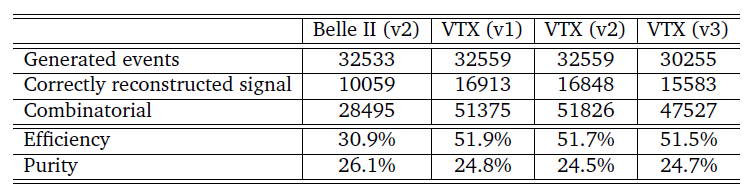
\includegraphics[scale=.9]{simulation_low_mom}
\caption{Reconstruction efficiency and purity for the the decay chain $B^{0} \rightarrow D^{*-}l^{+}\nu$, with $D^{*-} \rightarrow \bar{D}^{0} \pi^{-}_{soft}$ and $\bar{D}^{0} \rightarrow K^{+} \pi^{-}$, for the nominal Belle II detector at the intermediate background conditions and the nominal configuration of VTX in all three background scenarios.}
\label{fig:simulation_low_mom}
\end{figure}

We can see that the VTX reconstruction efficiency\footnote{Efficiency is defined as the ration between the number of correctly reconstructed signal events and the total number of candidates.}  in all three background hypotheses, results to be improved of almost a factor 1.7 with respect to the nominal Belle II, with comparable purity\footnote{} . Moreover efficiency remains practically stable in all background conditions, even in the most severe one.

This enhancement in tracking efficiency relies in particular on improved tracking efficiency for the $\pi_{soft}^{-}$ mesons, as we can see in~\autoref{fig:simulation_soft_pi}.


\begin{figure}[h!]
\centering
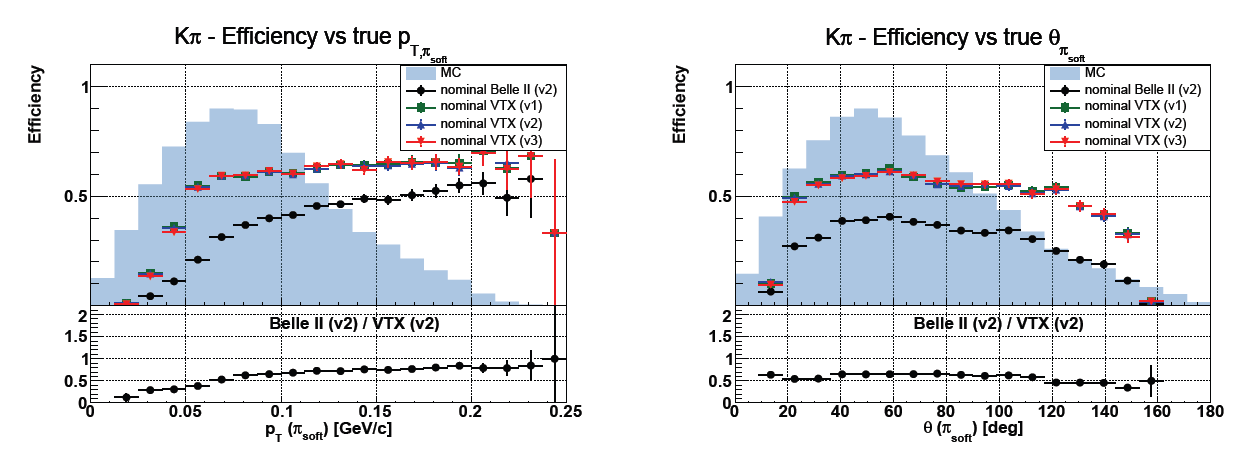
\includegraphics[scale=.53]{simulation_soft_pi}
\caption{Reconstruction efficiency of $B^{0} \rightarrow D^{*-}l^{+}\nu$ as a function of the transverse momentum of the $\pi_{soft}^{-}$ (from  $D^{*-} \rightarrow \bar{D}^{0} \pi^{-}_{soft}$) in the plot on the left and of the polar angle of the $\pi_{soft}^{-}$ on the right. 
The shaded blue histograms represents the momentum spectrum of the  $\pi_{soft}^{-}$.
The nominal Belle II geometry efficiency in the intermediate background scenario (\textbf{v2}) is represents by black dots and it is compared with the nominal VTX configuration in the optimistic (\textbf{v1}, green squares), medium (\textbf{v2}, blue upward pointing triangles) and pessimistic (\textbf{v3}, red downward
pointing triangles) background hypotheses. The bottom plots show the ration between nominale Belle II and nominal VTX in the \textbf{v2} background scenario.}
\label{fig:simulation_soft_pi}
\end{figure}

For all scenarios with nominal VTX, there is a powerful improvement for transverse momenta below 0.05 GeV/c, with respect to the nominal Belle II. Only for $p_{T}$ greater than 0.2 GeV/c the reconstruction efficiency of Belle II approach those of the VTX.\\

For $p_{T}$ higher than 0.3 GeV/c instead, the momentum resolution is dominated by the CDC and there is not a significant enhancement in track momentum resolution in the preceding example.

\subsection{Vertexing resolution}

The studies on vertexing performance have been conducted considering samples of one million $B^{0} \rightarrow J/\psi K_{S}^{0}$ events generated and reconstructed with all the aforementioned combinations.
The distributions of the decay vertex resolution $\sigma_{z}$ (i.e. the width of the distribution obtained considering the differences between the measured and the true simulated positions) along the \textit{z} axis of the B decay signal, are shown in~\autoref{fig:simulation_vertex}.

\begin{figure}[h!]
\centering
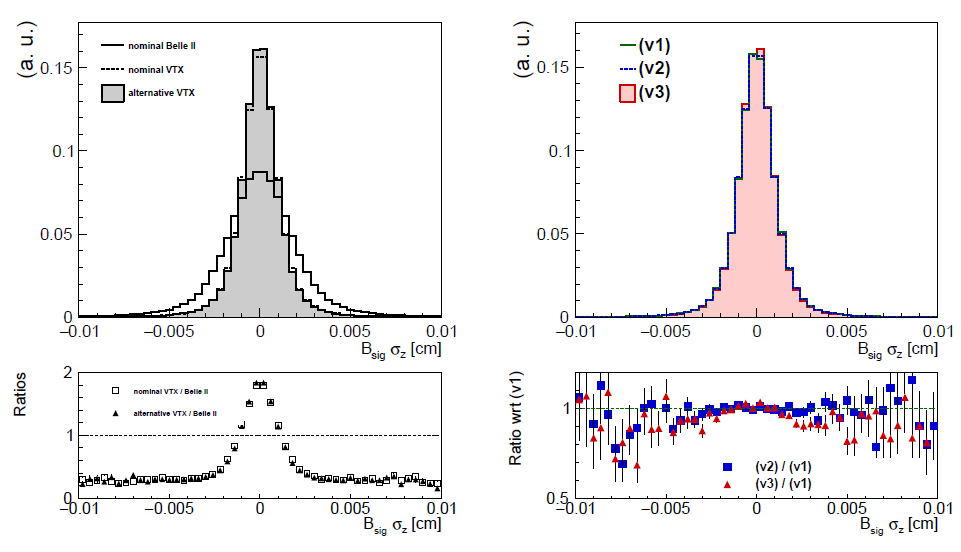
\includegraphics[scale=.65]{simulation_vertex}
\caption{On the left: comparison of the B decay vertex resolution along the \textit{z} axis in $B^{0} \rightarrow J/\psi K_{S}^{0}$ events for the nominal Belle II (solid line), nominal VTX (dotted line) and alternative VTX geometry (filled grey histogram). The bottom plot shows the ratio between the VTX geometries (empty squares the nominal one and filled triangles the alternative) and nominal Belle II. \\
On the right:  B decay vertex resolution along the \textit{z} axis for the nominal VTX geometry in the three background scenarios: optimistic \textbf{v1} (green solid line), intermediate \textbf{v2} (blue dotted line) and pessimistic \textbf{v3} (red filled histogram). The bottom plot represents the ratio between the two higher background scenarios and the optimistic one.}
\label{fig:simulation_vertex}
\end{figure}

In table~\ref{fig:simulation_vertex_table} a summary of the results that shows that the new geometries achieve a better resolution on the B decay vertex of about 35\% on average and they also do not suffer of any significant degradation as the background conditions varies, unlike the nominal Belle II configuration.


\begin{figure}[h!]
\centering
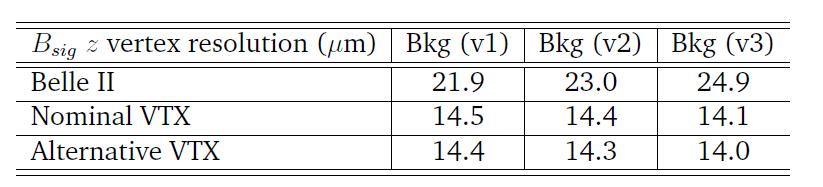
\includegraphics[scale=.8]{simulation_vertex_table}
\caption{$B_{sig}$ vertex resolution along the \textit{z} axis for the three detector geometry and the three background scenarios.}
\label{fig:simulation_vertex_table}
\end{figure}

The VTX geometries have been demonstrated to achieve better performance also for the vertexing resolution along the \textit{x} and \textit{y} axes. Also in these directions they turn out to be almost insensitive to the different levels of background.\\

Similar studies for the $K_{S}^{0}$ decay vertex resolution are displayed in~\autoref{fig:simulation_vertex_K} and in the same way, the upgraded geometries reach a better vertexing resolution with respect to the nominal Belle II detector without any sginifcant degradation as the backgrounds increase.
It is importan to notice that in the right plot there is a spurious effect that cause an apparent improvement of performance in the worst case scenario among those considered. This is due to the loss of reconstruction efficiency for candidates with large flight distance (thus affected by poorer vertex resolution).

\begin{figure}[h!]
\centering
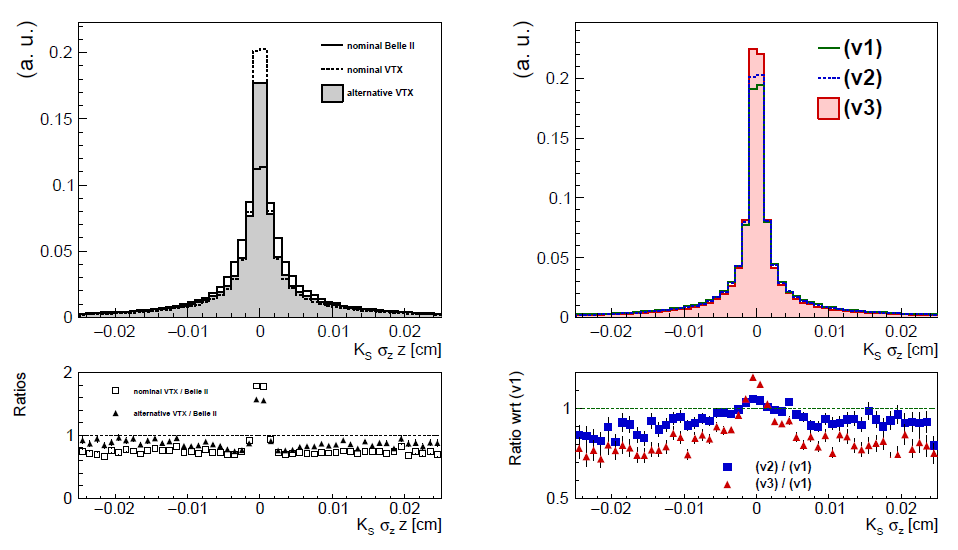
\includegraphics[scale=.65]{simulation_vertex_K}
\caption{On the left: comparison of the $K_{S}^{0}$ decay vertex resolution along the \textit{z} axis in $B^{0} \rightarrow J/\psi K_{S}^{0}$ events for the nominal Belle II (solid line), nominal VTX (dotted line) and alternative VTX (filled grey histogram). Thebottom plot shows the rattio between the VTX geometries (empty squares for the nominal and filled triangles for the alternative) and nominal Belle II detector. 
On the right: $K_{S}^{0}$ decay vertex resolution along the \textit{z} axis for the nominal VTX in the three background scenarios: optimistic \textbf{v1} (green solid line), intermediate \textbf{v2} (blue dotted line) and pessimistic \textbf{v3} (red filled histogram). The bottom plot represents the ratio between the two higher background scenarios and the optimistic one.}
\label{fig:simulation_vertex_K}
\end{figure}


%---------------------------------------------
%			3.3
%---------------------------------------------
\section{OBELIX chip design}

The VTX detector is designed with a single type sensor taylored to the specific needs of Belle II, called OBELIX (Optimized BELle II pIXel sensor) and currently under development, based on fast and high granular Depleted Monolithic Active Pixel Sensor (DMAPS). This new sensor design comes from an evolution of TJ-Monopix 2, whose characterization is the main topic of this thesis, and which will be discussed in chapter 5. Both of them are fabricated in a modified TowerJazz Semiconductor 180 $\mu$m CMOS process, that matches particularly well the Belle II requirements.
In particular its predecessor is equipped with four different flavors (\autoref{sec:flavors}), that are distinguished by different type of collection electrode coupling and some little difference in the circuit design. For now their characterization are ongoing and the final decision on which to use for Obelix has not been made. \\

\subsection{Sensor specification}

A schematic layout of the chip is shown in~\autoref{fig:obelix_scheme}. The size of the sensor is expected to be 3 x 1.9 $cm^{2}$, with an active area of 3 x 1.6 $cm^{2}$ and an additional part in the periphery of about 3 x 0.3 $cm^{2}$ dedicated to data pre-processing and triggering. The pixel pitches are designed to be from 30 $\mu$m to 40 $\mu$m in both direction. As a matter of fact staying in this range is necessary in order to achieve a spatial resolution below 15 $\mu$m, wihch is a requirement of the VTX upgrade program.

%REQUIRED RESOLUTION FROM CDR 15UM

\begin{figure}[h!]
\centering
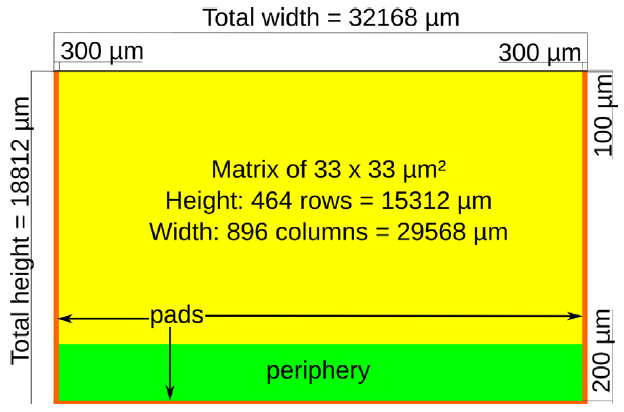
\includegraphics[scale=.7]{obelix_schematic}
\caption{OBELIX chip design.}
\label{fig:obelix_scheme}
\end{figure}

Moreover the sensor thickness has to be below 100 $\mu$m to respect the material budget constraint of 0.2\%$X_{0}$ and as consequence the depleted sensitive region should be lower than 50 $\mu$m, perfectly in agreement with the available thickness of MAPS  technology. 
To deal with the target hit rate of 120 MHz/$cm^{2}$, the timestamp clock signal can reach down to 25 ns, even if studies have demonstrated that a window of 100 ns (\textit{integration time}) is enough to limit to 320 Mbps the data throughput at the same expected hit rate. 
All topics faced above allow to realize a sensor with high granularity in both space and time.\\

With respect to TJ-Monopix 2, which is equipped with a triggerless column-drain readout without memory at the periphery, OBELIX must have a triggered readout architecture, in order to satisfy the needs of Belle II. Moreover the latency is fixed to 5(10) $\mu$s and it might operate up to 30 KHz trigger rate.

The expected power consumption instead, is expected to be about 200 mW$cm^{-2}$, a value which should allow air-cooling for the small area corresponding to the two inner layers and liquid coolant for the outer ones. 

%It is wort to mention that one of the specification of the sensor 

\begin{comment}
Tolerance to Total Ionizing Dose (TID) and Non Ionizing Energy Loss (NIEL)
fluence have been discussed already. But Single Event Effects (SEE) generated
by radiation might affect the sensor. Since no latchup (SEL) were observed in the
past operation years of Belle II, no specification is given. However Single Event
Upset (SEU) were observed and will be a concern to some extent, but are not yet
35 quantified. Consequently, the first specification is to ensure that the control system
allows resetting the sensor registers to the operational values at least every
few minutes. The actual frequency will be chosen after the measurement of the
SEU cross section with the OBELIX sensor and the comparison to the occurrence
distribution of large energy loss in the experiment.
\end{comment}

Its main design features are summarised in~\autoref{fig:obelix_features}.


\begin{figure}[h!]
\centering
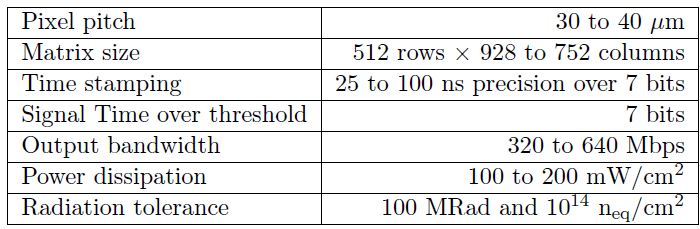
\includegraphics[scale=.7]{obelix_features}
\caption{Designed features of the OBELIX sensor.}
\label{fig:obelix_features}
\end{figure}

\begin{figure}[h!]
\centering
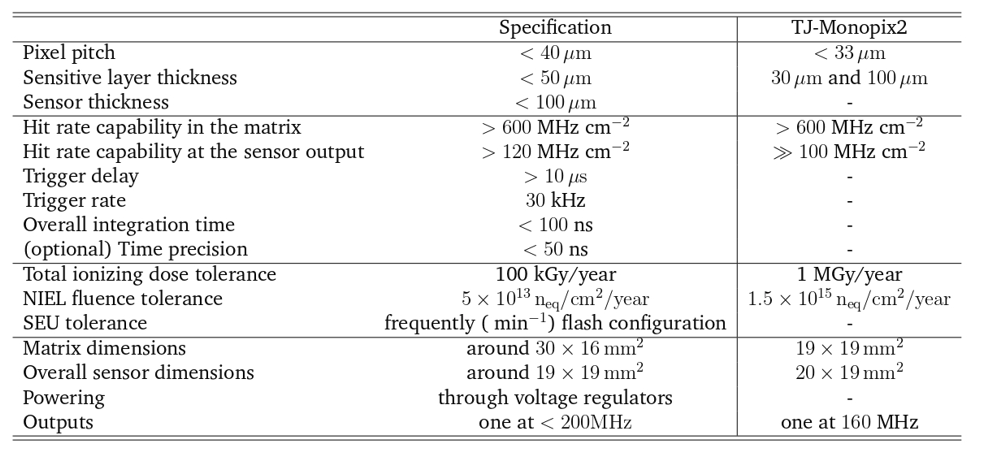
\includegraphics[scale=.6]{obelix_specification}
\caption{Comparison between OBELIX requirements and TJ-Monopix 2 features.}
\label{fig:obelix_specification}
\end{figure}

\subsection{Sensor implementation}

The technical implementation of the OBELIX sensor have to match all main features listed in table \ref{fig:obelix_features} .
As mentioned above, this new sensor is the development of Tj-Monopix 2, whose characteristics fit the Belle II requirements.\\

From Tj-Monopix 2 design, the pixel pitch of 33 x 33 $\mu m^{2}$ is maintained, as well as the layout of both digital and analogue parts. Also the Time-Over-Threshold method to digitized the signal is preserved, with a bus width of 7 bit, togheter with the column-drain readout architecture implemented for pairs of columns. Other features which will be explained in depth in chapter 5, have been conserved in the new design like the 3-bit register dedicated to the threshold tuning, but with a larger range of correction. 
Moreover to aim at the integration time of 100 $\mu$s, the clock frequency which defines the precision of ToT and BCID (that is the timestamp), has been decreased from 40 to 20 MHz. So the current baseline for OBELIX timestamp precision is 50 ns.

However two new modules are added to the implementation, related to the Belle II trigger: the Trigger Logic Unit (TRU) and the Track Trigger Transmitter (TTT). %that we will described in a few words.

\begin{description}
\item \textbf{Trigger Logic Unit (TRU)}
\end{description}

The TRU has to select the fired pixel information from the matrix, which are in-time with the triggers sent by the Belle II system. In more details, this module employs two stages of memory in order to manage the data coming from the pixel matrix (\autoref{fig:obelix_tru}). These components are design in order to minimize power dissipation and to optimize the efficiency even in severe operating conditions: maximum hit rate of 120 MHz$cm^{-2}$, 30 KHz of trigger rate and 10 $\mu$s of trigger delay.

\begin{figure}[h!]
\centering
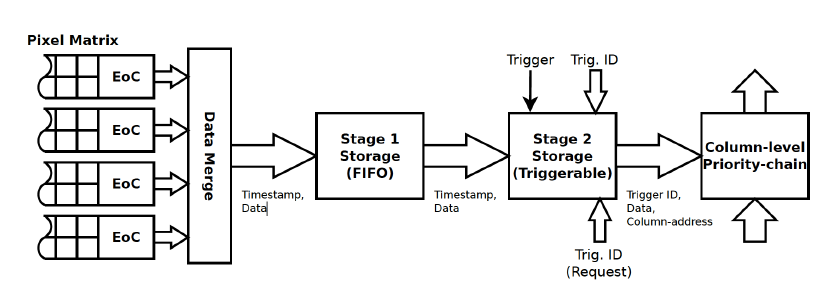
\includegraphics[scale=.8]{obelix_tru}
\caption{Schematic of the Trigger Logic Unit.}
\label{fig:obelix_tru}
\end{figure}

The first stage has to store the pixel information during the trigger delay (10 $\mu$s). The second memory instead, has the task to compare the BCID of the fired pixel with each trigger time information buffered in a dedicated global memory which keeps track of received triggers. When they have a match, the pixel data is transferred to the Transmission Unit (TXU). Considering the BCID precision time, the time integration of the OBELIX sensor becomes 100 ns.

%This strategy accounts for the possibility that a physics hit associated to a trigger is timestamped with a later BCID due for instance to timewalk effect.


\begin{description}
\item \textbf{Track Trigger Transmitter (TTT)}
\end{description}

The TTT module divides the matrix in 8 logic regions (this value is still under study) and generates a one-byte word depending on the region that is fired. It is expected taht this information could be transmitted to trigger system within 100 ns and along a line of transmission parallel to the main data output of the sensor. 
This component behaviour is still under study and it needs of further simulations in correlation with the whole VTX system.


\begin{description}
\item \textbf{Control Unit (CRU) and power dissipation}
\end{description}

The OBELIX sensor, as well as TJ-Monopix 2, is configured by several registers which allow to set crucial features for its operation like threshold settings, masked pixels, time response of the pixel and so on but also define its power consumption. The Control Unit is responsible for receiving these instructions about the configuration and the trigger information and at the same time sending out data coming from TXU module.

For what concern power dissipation, there are three main features which have the greatest impact: the biasing current flowing into the in-pixel amplifier (i.e. \textit{$I_{BIAS}$}), the BCID clock frequency (on which depends the timestamping precision) and the hit rate. In~\autoref{fig:obelix_power_cons} is shown the estimations of power dissipation as these parameters vary.


\begin{figure}[h!]
\centering
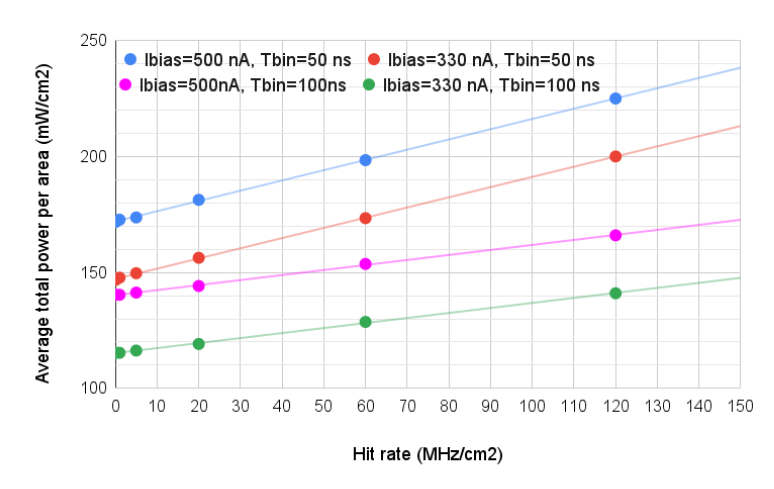
\includegraphics[scale=.8]{obelix_power_cons}
\caption{OBELIX sensor power dissipation depending on the front edn current (\textbf{$I_{bias}$}, the BCID frequency (\textbf{tbin}) and the hit rate).}
\label{fig:obelix_power_cons}
\end{figure}

As we can see, the power consumption at the maximum hit rate of 120 MHz$cm^{-2}$ exceeds by little more than 10\% the power budget of 200 mW$cm^{-2}$ considering the higher precision for the timestamp of 50 ns. Therefore to stay within the power budget it is necessary to find a compromise: reducing timing precision by worsening the BCID precision to 100 ns or decreasing the pre-amplifier biasing current causing a degradation of the time walk.


The first version of the sensor, called OBELIX-1, is being designed and the submission for fabrication is planned in the last month of 2023. A second improved version, OBELIX-2, will be designed based on performance studies on the first version and it is expected that it will be the final sensor needed for the experiment.




%---------------------------------------------
%		BIBLIOGRAFIA
%---------------------------------------------

%TVX ARTICLE
%CDR
%LUDO
%VTX proposal


%---------------------------------------------
%		COMMENT
%---------------------------------------------
